\documentclass[a4paper, 11pt, twoside]{article}

\usepackage[english]{babel}
\usepackage[latin1]{inputenc}

\usepackage{graphicx,float}
\usepackage{subfigure}
\usepackage{xcolor}
\usepackage{tabularx}
\usepackage{pgfplots}
\usepackage{type1cm}
\usepackage{amssymb, amsthm, amsmath}
\usepackage{listings}
\usepackage{pgf}
\usepackage{url}
\usepackage{hyperref}
\usepackage{tikz}

\usepackage{makeidx}
\makeindex

\setlength{\parindent}{0em}
\setlength{\oddsidemargin}{0.0cm}
\setlength{\evensidemargin}{0.0cm}
\setlength{\textheight}{24.0cm}
\setlength{\topmargin}{-1.0cm}
\setlength{\footskip}{1.5cm}
\setlength{\textwidth}{15.5cm}

\renewcommand*\familydefault{\sfdefault}
\newcommand{\dd}{\mathrm{d}}
\newtheorem{problem}{Problem}[section]
\newtheorem{theorem}{Theorem}[section]
\newtheorem{remark}{Remark}[section]

\begin{document}
\pagestyle{empty}
%\documentclass[a4paper]{article}

%\usepackage{pgf}
%\usepackage{graphicx}
%\usepackage{pifont}
%\usepackage{type1cm}

\setlength{\textwidth}{14cm}
\setlength{\oddsidemargin}{1cm}

%\begin{document}

\pagestyle{empty}

%%%%%%%%%%%%%%%%%%%%%%%%%%%%%%%%%%%%%%%%
%%%%%%%%%%%%%%%%%%%%%%%%%%%%%%%%%%%%%%%%
%%%%%%%%%%%%%%%%%%%%%%%%%%%%%%%%%%%%%%%%

\newcount \Z
\Z=20

%%% logos %%%

%%% NUMHPC %%%
\newlength{\numhpclogox}
\setlength{\numhpclogox}{\paperwidth} % 20/210ths of the paperwidth
\divide\numhpclogox by 210
\multiply\numhpclogox by 100

\newlength{\numhpclogoy}
\setlength{\numhpclogoy}{\paperheight} % 270/297ths of the paperwidth
\divide \numhpclogoy by 297
\multiply \numhpclogoy by -235

\newlength{\numhpclogoheight}
\setlength{\numhpclogoheight}{\paperheight} % 270/297ths of the paperwidth
\divide\numhpclogoheight by 297
\multiply\numhpclogoheight by 20

%%% KIT %%%
\newlength{\kitlogox}
\setlength{\kitlogox}{\paperwidth} % 20/210ths of the paperwidth
\divide\kitlogox by 210
\multiply\kitlogox by 0

\newlength{\kitlogoy}
\setlength{\kitlogoy}{\paperheight} % 270/297ths of the paperwidth
\divide \kitlogoy by 297
\multiply \kitlogoy by -230

\newlength{\kitlogoheight}
\setlength{\kitlogoheight}{\paperheight} % 270/297ths of the paperwidth
\divide\kitlogoheight by 297
\multiply\kitlogoheight by 15


%%% EMCL %%%
\newlength{\emcllogox}
\setlength{\emcllogox}{\paperwidth} % 20/210ths of the paperwidth
\divide\emcllogox by 210
\multiply\emcllogox by 28

\newlength{\emcllogoy}
\setlength{\emcllogoy}{\paperheight} % 270/297ths of the paperwidth
\divide \emcllogoy by 297
\multiply \emcllogoy by -160

\newlength{\emcllogoheight}
\setlength{\emcllogoheight}{\paperheight} % 270/297ths of the paperwidth
\divide\emcllogoheight by 297
\multiply\emcllogoheight by 20

%%% HIFLOW %%%
\newlength{\hiflowlogox}
\setlength{\hiflowlogox}{\paperwidth} % 20/210ths of the paperwidth
\divide\hiflowlogox by 210
\multiply\hiflowlogox by 28

\newlength{\hiflowlogoy}
\setlength{\hiflowlogoy}{\paperheight} % 270/297ths of the paperwidth
\divide \hiflowlogoy by 297
\multiply \hiflowlogoy by -160

\newlength{\hiflowlogoheight}
\setlength{\hiflowlogoheight}{\paperheight} % 270/297ths of the paperwidth
\divide\hiflowlogoheight by 297
\multiply\hiflowlogoheight by 33

%%%%%%%%%%%%%%%%%%%%%%%%%%%%%%%%%%%%%%%%
%%%%%%%%%%%%%%%%%%%%%%%%%%%%%%%%%%%%%%%%
%%%%%%%%%%%%%%%%%%%%%%%%%%%%%%%%%%%%%%%%

%%% NUMHPC %%%
%%\pgftext[bottom, left, at={\pgfpointadd{\pgfpoint{0pt}{0pt}}{\pgfpoint{\numhpclogox}{\numhpclogoy}}}]{\includegraphics[totalheight=\numhpclogoheight]{numhpc}}

%%% KIT %%%
%%\pgftext[bottom, left, at={\pgfpointadd{\pgfpoint{0pt}{0pt}}{\pgfpoint{\kitlogox}{\kitlogoy}}}]{\includegraphics[totalheight=\kitlogoheight]{kitlogo}}

%%% EMCL %%%
\pgftext[bottom, left, at={\pgfpointadd{\pgfpoint{0pt}{0pt}}{\pgfpoint{\hiflowlogox}{\hiflowlogoy}}}]{
\includegraphics[totalheight=\hiflowlogoheight]{HF3_color}}

%%% horizontal lines %%%
\pgfline{\pgfxy(-1pt,0.1pt)}{\pgfxy(15pt,0.1pt)}
\pgfline{\pgfxy(-1pt,-21.4pt)}{\pgfxy(15pt,-21.4pt)}
%%\pgfline{\pgfxy(-1pt,-22.4pt)}{\pgfxy(15pt,-22.4pt)}

%%% EMCL text %%%
\pgftext[bottom, left, at={\pgfpointadd{\pgfpoint{0pt}{0pt}}{\pgfpoint{0cm}{1cm}}}]{{\LARGE{{\bf Tutorial}}}}

%%% EMCL web %%%
\pgftext[bottom, left, at={\pgfpointadd{\pgfpoint{0pt}{0pt}}{\pgfpoint{10.5cm}{-21.7cm}}}]{{\fontsize{13}{10}\selectfont{} http://www.hiflow3.org/}}

\hspace{2cm}
\begin{picture}(0,0)(-250,-25)

\includegraphics[scale=.22]{emcl.pdf} 
\end{picture}

%%% author %%%
\pgftext[bottom, left, at={\pgfpointadd{\pgfpoint{0pt}{0pt}}{\pgfpoint{0cm}{-4cm}}}]{{
\begin{parbox}{13cm}{
\begin{center}\fontsize{12}{30}\selectfont{} J. Kratzke, K. Mang
\end{center}}
\end{parbox}}}

%%% title %%%
\pgftext[bottom, left, at={\pgfpointadd{\pgfpoint{0pt}{0pt}}{\pgfpoint{0cm}{-7.5cm}}}]{{
\begin{parbox}{13cm}{
%%\begin{center}\fontsize{18}{30}\selectfont{} \bf Using HiFlow$^3$ for solving the
\begin{center}\fontsize{22}{30}\selectfont{} \bf Aortic Blood Flow Simulation
\end{center}}
\end{parbox}}}

%%% date %%%
\pgftext[bottom, left, at={\pgfpointadd{\pgfpoint{0pt}{0pt}}{\pgfpoint{0cm}{-16.4cm}}}]{{
\begin{parbox}{13cm}{
\begin{center}\fontsize{12}{24}\selectfont{} 
\vspace{5cm}
\textit{modified on \today}\\ 
\vspace{6.5cm}
\hspace{6cm}\textit{Version 2.0}
\end{center}}
\end{parbox}}}

%fhfh \hfill sjdh

%\end{document}


\tableofcontents

\newpage
\pagestyle{plain}
\framebox[15.5cm]{\parbox[c][2.3cm]{14.5cm}{
{\fontsize{19}{19}\selectfont{} \bf{Computational Fluid Dynamics:\\ Aortic Blood Flow Simulation}
}}}
\vspace{0.5cm}
\section{Introduction}
Cardiovascular disease is a large cause of death worldwide,
which is responsible for more than half of mortality in the developed
countries. The examination of biomechanical dynamics in the
cardiovascular system can provide crucial information on cardiovascular
physiology and pathology. Hemodynamic parameters, such as blood velocity
and pressure distribution, as well as vessel wall stress and strain have
shown to correlate with the development of cardiovascular disease. Two
of the most severe pathologies are aneurysm growth or aortic dissection.
Yet, how to assess development and risk of cardiovascular disease in
many cases remains an open question.\\

Medical imaging and mechanical experiments on blood flow have driven the
mathematical modeling of hemodynamics to better understand
cardiovascular physiology and pathology. Numerical simulations based on
mathematical models and calibrated patient-individually can generate
information complementary to medical imaging. An example is
given by computational fluid dynamics (CFD) enabling spatially and resolved visualization
in space and time of flow and pressure distribution.

\subsection{HiFlow$^3$}
HiFlow$^3$ is a multi-purpose finite element software providing powerful tools for efficient and accurate solution of 
a wide range of problems modeled by partial differential equations (PDEs). Based on object-oriented concepts and the full
capabilities of C++ the HiFlow$^3$ project follows a modular and generic approach for building efficient parallel 
numerical solvers. It provides highly capable modules dealing with the mesh setup, finite element spaces, degrees 
of freedom, linear algebra routines, numerical solvers, and output data for visualization. Parallelism - 
as the basis for high performance simulations on modern computing systems - is introduced on two levels: 
coarse-grained parallelism by means of distributed grids and distributed data structures, and fine-grained parallelism
by means of platform-optimized linear algebra back-ends.

\subsection{How to Use the Tutorial?}
You find the example code (blood\_flow\_tutorial.cc, blood\_flow\_tutorial.h) and a parameter file for the first numerical 
example (blood\_flow\_tutorial.xml).
The geometry data (*.inp, *.vtu) is stored in the folder \verb'/hiflow/examples/data'.

\subsubsection{Using HiFlow$^3$ as a Developer}\label{sectiondeveloper}
First build and compile HiFlow$^3$. Go to the directory \verb'/build/example/blood_flow', 
where the binary \textbf{blood\_flow\_tutorial} is stored. Type \textbf{./blood\_flow\_tutorial}, 
to execute the program in sequential mode. To execute in parallel mode \index{program!executing in parallel} 
with four processes, type \textbf{mpirun -np 4 ./blood\_flow\_tutorial}. 
In both cases, you need to make sure that the default parameter file blood\_flow\_tutorial.xml 
is stored in the same directory as the binary, and that the geometry data specified in the parameter file is stored 
in \verb'/hiflow/examples/data'. 
Alternatively, you can specify the path of your own xml-file with the name of your xml-file in the comment line,
i.e. \textbf{./blood\_flow\_tutorial} \verb'/"path_to_parameterfile"/"name_of_parameterfile".xml'.
\\

\section{Mathematical Setup}

\subsection{Problem formulation}\label{intro}
Blood is a suspension of about 45\% blood cells, which cause a shear-thinning behavior. 
They arrange themselves in rolls at low shear rates, which break
open at higher velocities. In large arteries this effect is relatively
small, such that blood flow can be modeled as Newtonian with constant
viscosity. An incompressible Newtonian fluid can be described by the
Navier-Stokes equations.\\

We consider the simulation of instationary laminar blood flow in a three-dimensional geometry. 
To obtain a unique solution, the formulation of the problem is completed by setting appropriate
conditions on the boundary of the respective geometries. We have to distinguish three different conditions, namely, 
(\ref{NR1}) velocity conditions at  $\Gamma_{\text{vel}}$, 
(\ref{NR2}) pressure conditions $\Gamma_{\text{p}}$
and (\ref{NR3}) the no-slip condition
at the vessel wall $\Gamma_0$.
We define the initial boundary value problem for the unknown velocity field $v = (v_1(x,t), v_2(x,t), v_3(x,t))^T$ 
and the unknown pressure $p = p(x,t)$ with a three-dimensional vector $x \in \Omega$ as follows:

\begin{align}
\label{eq:NS_strong1}\tag{1a}
\frac{\partial v}{\partial t} + (v \cdot \nabla ) v -\nu \Delta v + \frac{1}{\rho} \nabla p &= f, \quad \text{ in } \Omega \times \mathcal {I},\\
\label{eq:NS_strong2}\tag{1b}
	 \nabla \cdot v &= 0, \quad \text{ in } \Omega\times \mathcal {I},\\
 \label{NR1}\tag{1c}
v &= g, \quad \text{ on } \Gamma_{\text{vel}} \times \mathcal {I},\\ 
\label{NR2}\tag{1d}
(- \mathcal{I} \frac{p}{\rho} + \nu \nabla v) \cdot n &= \frac{P}{\rho}, \quad \text{ on } \Gamma_{\text{p}} \times \mathcal {I},\\
 \label{NR3}\tag{1e}
 	v &= 0, \quad \text{ on } \partial\Omega \backslash (\Gamma_{\text{vel}} \cup \Gamma_{\text{p}})=:\Gamma_0,  
 \end{align}   

where $\Omega$ is the domain specified in figure \ref{geometries} and $\mathcal {I}$ is a time interval.
The kinematic viscosity\index{viscosity} $\nu$ is a material constant and the mass
density\index{density} $\rho$ is also assumed to be constant due to the incompressibility of the fluid. In case of blood, the viscosity is approximately $4 \times 10^{-6} \frac{m^2}{s}$ and the density $1,060 \frac{g}{cm^3}$.
$n = n(x)$ is the outer normal vector on $ \partial \Omega$ and $ I \in \mathbb {R} ^ {3 \times 3} $ the unit matrix and $g:\Gamma_{\text{in}} \times \mathcal {I} \rightarrow \mathbb{R}$ is a given velocity data.
The right hand side $f$ accounts for the possible action of external forces like gravity.
In the case of human blood flow, we can assume $f = 0$.\\
We have to consider that the nonlinear convection term $(v\cdot  \nabla)v$ may develop turbulences, if we have high Reynold numbers.
In the aorta we are dealing with a Reynold number of around $3500$.\\

First we will test our implementation with a simple three dimensional tube as in figure \ref{geometries} (left), then we will consider the human aorta with real data as given in figure \ref{geometries} (right).

\begin{figure}[!h]
\centering
\begin{minipage}{0.45\textwidth}
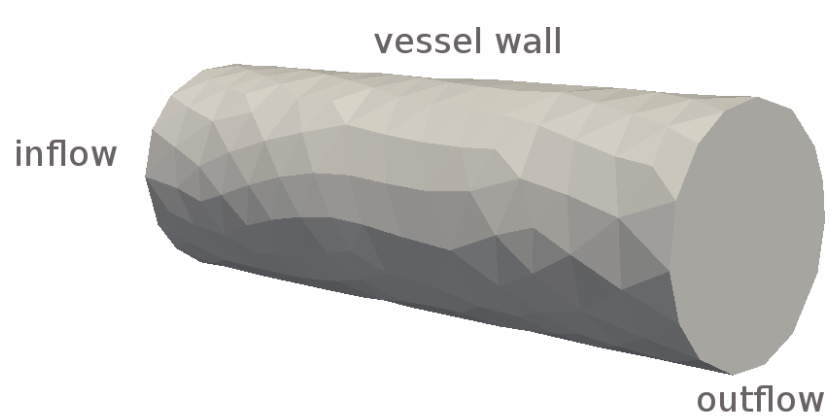
\includegraphics[width=\textwidth]{fig/channel_gray.png}
\end{minipage}
\hspace{1.0cm}
\begin{minipage}{0.33\textwidth}
  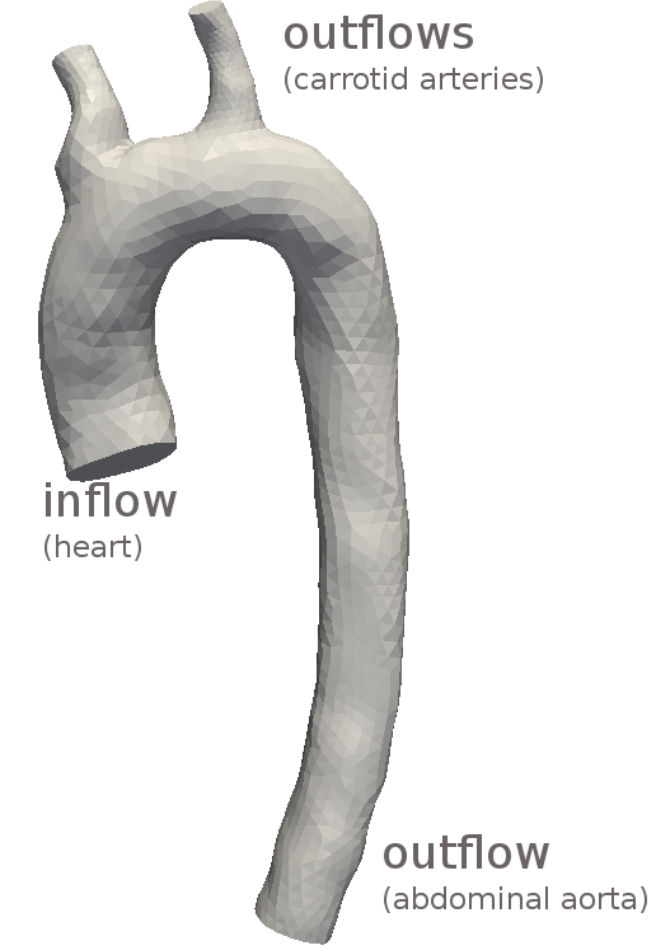
\includegraphics[width=\textwidth]{fig/aorta_gray.png}
  \end{minipage}
\caption{Simple test geometry (left) and a geometry of a human aorta in 3D (right).}
\label{geometries}
\end{figure}

\subsubsection{Velocity Dirichlet Boundary Conditions from measurement data}
We assume the vessel wall to be rigid, which implies that we have $v=0$ on $\Gamma_0$. This is also called no-slip boundary condition.\\
We set the distribution of velocities at the velocity boundaries by means of a Poiseuille profile:
\begin{align}
 v(r,t) = \left(\left(\frac{r}{R}\right)^b-1\right)\ a\ Q(t),\label{poiseuille}
\end{align}
where $r$ ist the radial distance from the centerline, $R$ the radius of the opening, $a:= \frac{b+2}{b \pi R^2}$ and $Q(t)$ denotes the flow rate given from measured physiological data.
For a constant laminar flow through a straight tube, it can be analytically derived, that (\ref{poiseuille}) with $b=2$ is the solution for the velocity field of the incompressible Navier-Stokes equations.
\subsubsection{Pressure Neumann Boundary Condition}
Aortic outflow boundaries can be modeled by the Windkessel model designed
in the late 1800's by Otto Frank. He described the heart and the systemic arterial system as a closed hydraulic circuit. In his analogy,
the circuit contained a water pump connected to a chamber, filled with water except for a pocket
of air. As it is pumped, the water compresses the air, which in turn pushes the water out of the
chamber. This analogy resembles the mechanics of the heart. Windkessel models are commonly
used to represent the load undertaken by the heart during the cardiac cycle. It relates
blood pressure and blood flow in the aorta, and characterizes the arterial compliance, peripheral 
resistance and the inertia of the blood flow.\\
The arterial compliance refers to the elasticity 
and extensibility of the major artery during cardiac cycle.The peripheral resistance
refers to the flow resistance encountered by the blood as it flows
through the systemic arterial system and the inertia simulates the inertia of the blood as it is cycled through the heart.\\

The simplest of the Windkessel models demonstrating the hemodynamic state is the $2$-Element model which takes into
account the effect of arterial compliance and total peripheral resistance.\\
The flow of blood from the heart $Q(t)$ is analogous to that of current flowing in the circuit and the blood pressure in the aorta
$P(t)$ is modeled as a time-varying electric potential. \\
The theoretical modeling is given as:
\begin{align}
 Q(t) = \frac{P(t)}{R} + C \frac{dP(t)}{dt},
\end{align}
with $C$ the compliance and $R$ the resistance.
Via the difference quotient we get for every timestep $k \in [0,T]$
\begin{align}
 Q_{k-1}=\frac{1}{R} P_k + C \frac{P_k-P_{k-1}}{\partial t}.
\end{align}
Out of this we are able to to get a discretized value of the new pressure value $P_k$ in any timestep:
\begin{align}
 P_k = \frac{R \partial t}{\partial t + CR}\ Q_{k-1} - \frac{CR}{\partial t + CR}\ P_{k-1}.
\end{align}
For more details see \cite{windkessel}.\\

First we will test our simulation with a simple cubic tube, which has one Poiseuille-inflow boundary and one Windkessel
outflow boundary condition.\\
If we consider in a next step the real aorta geometry out of patient data, we have as well one Poiseuille-inflow boundary,
but three outflow boundaries. 
The two Carotis outflows can be modeled as Poiseuille-outflow boundaries, the outflow of the abdominal aorta as a Windkessel-outflow boundary.\\

\subsection{Solving the nonlinear problem with Newton's method}\index{Newton's method}
The nonlinear term $(v\cdot \nabla)v$ turns the Navier-Stokes equation\index{equation!Navier-Stokes}\index{equation!nonlinear} (\ref{eq:NS_strong1}) into a nonlinear equation. One possibility 
to solve a nonlinear problem is using iterative Newton's method, for details we refer to the flow tutorial \cite{tutorial}.

\subsection{Weak Formulation}\index{weak formulation}
To solve a problem using finite element methods we take the variational formulation of the problem into account. 
It can be derived by multiplying the equation with test functions, integrating over the domain, applying integration by parts and the Gauss theorem, as it is described in the 
classical Navier-Stokes tutorial \cite{tutorial}. 

Let us have a closer look at the pressure Neumann boundary condition (\ref{NR3}):
\begin{align}
(- \mathcal{I} \frac{p}{\rho} + \nu \nabla v) \cdot n &= \frac{P_i}{\rho},\ i=1,2,3,..,m
\end{align}

where $P_i$ are given by the Windkessel model.
To establish this boundary we have the following variational formulation:\\
With given $P_i(t) ,\ i=1,2,..,m,$ find $(v,p) \in L^2(0,T;H_0^1(\Omega)) \times L^2(0,T;L^2(\Omega))$ such that for all $\varphi \in H^1(\Omega)$ and $\psi \in L^2(\Omega)$ holds
\begin{align}
 (\frac{\partial v}{\partial t},\varphi) + (v \cdot \nabla v,\varphi) + \nu (\nabla v,\nabla \varphi) + \frac{1}{\rho}(p,\nabla \cdot \varphi) =& - \sum_{i=1}^m \frac{P_i}{\rho} \int_{\Gamma_i} \varphi \cdot n d\gamma,\\\label{weak}
 (\nabla \cdot v,\psi) =&\ 0.
\end{align}
This formulation ensures that the mean pressure is a constant normal stress on the artificial boundaries $\Gamma_i$.
For more details see \cite{cardio}.

\subsection{Streamline diffusion}
For higher Reynolds numbers as in our case around $Re=3500$, we need to stabilize the slightly convection dominated flow problem.
Therefore, we use a streamline diffusion scheme as described in \cite{rannacher}. The idea is to introduce artificial diffusion acting only in the direction of 
transport while conserving the second-order accuracy of the FEM-discretization.
We write the discrete variational formulation as follows:\\
Find $v_h \in V_h^{in} + H_h$ and $p_h \in L_h$ such that
\begin{align*}
 (\frac{\partial v_h}{\partial t},\varphi_h) + (v_h \cdot \nabla v_h,\varphi_h) + \nu (\nabla v_h,\nabla \varphi_h) + \frac{1}{\rho}(p_h,\nabla \cdot \varphi_h) + s_h(\{v_h,p_h\},\{\varphi_h,\psi_h\}) = 0
\end{align*}
$\forall \{\varphi_h, \psi_h\} \in H \times L_h$, where,
\begin{align*}
s_h(\{v_h,p_h\},\{\varphi_h,\psi_h\}) = \sum_{k \in \mathbb{T}_h} \delta_K (v_h \cdot \nabla v_h, v \cdot \nabla \varphi)_K\}.
\end{align*}
The discretization parameter $\delta_K$ is set to
\begin{align*}
\delta_K = \frac{h^2}{6\nu + h |v|_K}.
\end{align*}
$s_h$ stabilizes the convection term. Because of the use of $P_2/P_1$ Taylor Hood elements, we do not need stabilization for regularization as
$P_2/P_1$ Taylor Hood elements itself fulfill naturally an inf-sup condition.

\subsection{Wall shear stress}\label{wss}
A recent review on methods of finite element analysis pointed out that simulations of aortic biomechanics have the potential to support individual assessment of risk factors. 
In particular, occurring low or high wall shear stress, computed by computational fluid dynamics, can indicate conditions of increased risk. For more detail see \cite{cardio}. 
The wall shear stress is defined as
\begin{align*}
\tau = |\rho \nu (\nabla v + \nabla v^T) \cdot n|
\end{align*}
We consider the magnitude of the wall shear stress which is exerted by the fluid flow field on the vessel-wall with normal vector $n$. \\

\section{The Commented Program}

\subsection{Preliminaries}
HiFlow$^3$ is designed for high performance computing on massively parallel machines. 
So it applies the Message Passing Interface (MPI)\index{Message Passing Interface (MPI)}\index{MPI} library specification for message-passing, see sections \ref{main}, \ref{run}, \ref{read-mesh}. 
The blood flow tutorial needs following two input files:
\begin{itemize}
\item A parameter file: The parameter file is an xml-file, which contains all parameters needed to execute the program. It is read in by the program. Parameters for example defining the termination condition of the nonlinear and linear solver are listed as well as parameters needed for the linear algebra. 
It is not necessary to recompile the program, when parameters in the xml-file are changed. 
it is your decision which example you want to execute. First you can use the parameter file blood\_flow\_tutorial\_channel.xml, see section \ref{sectionparameter file}, which contains the parameters of the simple benchmark numerical example, see section \ref{sectionChannel}.\\
This file is stored in \verb'/hiflow/examples/blood_flow/'. To execute the second example to simulate the flow in the aorta, see section \ref{sectionAorta},
you have to run the code with the parameter file blood\_flow\_tutorial\_aorta.xml, which is stored in the same folder.
\item Geometry data\index{geometry data}: The file containing the geometry is specified in the parameter file. 
\end{itemize}

\subsection{Parameter File}\index{parameter file}\label{sectionparameter file}
The needed parameters are initialized in the parameter file blood\_flow\_tutorial\_channel.xml.
\begin{lstlisting}[language=C++, basicstyle={\footnotesize, \ttfamily}, keywordstyle=\color{blue}, numbers=none, tabsize=4]
<Param>
  <OutputPrefix>blood_flow_tutorial_channel</OutputPrefix>
  <Mesh>
    <Filename>poiseuille_channel_res1.vtu</Filename>
    <InitialRefLevel>0</InitialRefLevel>
  </Mesh>
  <LinearAlgebra>
    <NameMatrix>CoupledMatrix</NameMatrix>
    <NameVector>CoupledVector</NameVector>
    <Platform>CPU</Platform>
    <Implementation>Naive</Implementation>
    <MatrixFormat>CSR</MatrixFormat>
  </LinearAlgebra>
  <FlowModel>
    <Density>3.0</Density>
    <Viscosity>1.0e-3</Viscosity>
    <StabilizationFactor>0.</StabilizationFactor>
  </FlowModel>
  <FiniteElements>
    <VelocityDegree>2</VelocityDegree>
    <PressureDegree>1</PressureDegree>
  </FiniteElements>
  <Instationary>
    <Timestep>0.1</Timestep>
    <Endtime>5.0</Endtime>
    <Theta>0.5</Theta>
    <SmoothStartTime>0.5</SmoothStartTime>
    <Period>1.0</Period>
    <VisualizationInterval>10</VisualizationInterval>
  </Instationary>
  <Boundary>
    <WallMaterial>1</WallMaterial>
    <NumberOfPoiseuilleBoundaries>1</NumberOfPoiseuilleBoundaries>
      <Poiseuille_0>
        <Material>3</Material>
        <Center>0 0 0</Center>
        <Normal>0 -1 0</Normal>
        <Radius>0.5</Radius>
        <Exponent>2</Exponent>
        <TimeStamps>0 0.1 0.2</TimeStamps>
        <FlowRates>1 1 1</FlowRates>
      </Poiseuille_0>
    <NumberOfWindkesselBoundaries>0</NumberOfWindkesselBoundaries>
  </Boundary>
  <NonlinearSolver>
    <Name>Newton</Name>
    <MaxIterations>100</MaxIterations>
    <AbsTolerance>1.e-9</AbsTolerance>
    <RelTolerance>1.e-9</RelTolerance>
    <DivTolerance>1.e5</DivTolerance>
    <ForcingStrategy>EisenstatWalker1</ForcingStrategy>
    <InitialForcingValue>1.e-2</InitialForcingValue>
    <MaxForcingValue>0.9</MaxForcingValue>
    <EW2Gamma>1.0</EW2Gamma>
    <EW2Alpha>1.0</EW2Alpha>
    <DampingStrategy>Armijo</DampingStrategy>
    <InitialDampingValue>1.0</InitialDampingValue>
    <MinimalDampingValue>1.e-4</MinimalDampingValue>
    <ArmijoDecrease>0.5</ArmijoDecrease>
    <SufficientDecrease>1.e-4</SufficientDecrease>
    <MaxDampingIterations>10</MaxDampingIterations>
  </NonlinearSolver>
  <LinearSolver>
    <Name>GMRES</Name>
    <MaxIterations>1000</MaxIterations>
    <AbsTolerance>1.e-9</AbsTolerance>
    <RelTolerance>1.e-3</RelTolerance>
    <DivTolerance>1.e6</DivTolerance>
    <SizeBasis>100</SizeBasis>
    <Preconditioning>ILUPP</Preconditioning>
     <ILUPP>
      <PreprocessingType>0</PreprocessingType>
      <PreconditionerNumber>11</PreconditionerNumber>
      <MaxMultilevels>20</MaxMultilevels>
      <MemFactor>0.8</MemFactor>
      <PivotThreshold>2.75</PivotThreshold>
      <MinPivot>0.05</MinPivot>
     </ILUPP>
  </LinearSolver>
</Param>
\end{lstlisting}

\subsection{Main Function}\label{main}\index{MPI}
The main function starts the simulation of the flow problem (blood\_flow\_tutorial.cc).

\begin{lstlisting}[language=C++, basicstyle={\footnotesize, \ttfamily}, keywordstyle=\color{blue},  numbers=none, tabsize=4]
int main ( int argc, char** argv )
{
    MPI_Init ( &argc, &argv );

    // Set default parameter file
    std::string param_filename ( PARAM_FILENAME );
    if ( argc > 1 )
        param_filename = argv[1];
    try
    {
        BloodFlowTutorial app ( param_filename );
        app.run ( );
    }
    catch ( std::exception& e )
    {
        std::cerr << "\nProgram ended with uncaught exception.\n";
        std::cerr << e.what ( ) << "\n";
        return -1;
    }
    MPI_Finalize ( );
    return 0;
}
\end{lstlisting}

\subsection{Member Functions}
Following member functions are components of the Navier-Stokes equation tutorial: 
\begin{itemize}
 \item run()
 \item EvalFunc(const CVector\& newton\_sol, CVector* res)
 \item EvalGrad(const CVector\& newton\_sol, CMatrix* jac)
 \item read\_mesh()
 \item prepare\_parameters()
 \item prepare\_space()
 \item prepare\_solver()
 \item prepare\_bc()
 \item calculate\_spline(int bdy\_id)
 \item evaluate\_spline(int bdy\_id, Scalar current\_time)
 \item run\_time\_loop()
 \item solve()
 \item evaluate()
 \item evaluate\_bdy\_flowrate(const int bdy\_material)
 \item evaluate\_bdy\_pressure(const int bdy\_material)
 \item visualize()
\end{itemize}

\subsubsection{run()}\index{MPI}\label{run}
The member function run() calls the functions solve() and visualize() to solve the stationary flow problem and to generate the  data for the visualization.The function is defined in the class FlowTutorial (blood\_flow\_tutorial.cc).

\begin{lstlisting}[language=C++, basicstyle={\footnotesize, \ttfamily}, keywordstyle=\color{blue},  numbers=none, tabsize=4]
void BloodFlowTutorial::run ( )
{
    simul_name_ = params_["OutputPrefix"].get<std::string>( );

    // Log Output on console
    LogKeeper::get_log ( "info" ).set_target ( &std::cout );
    // std::ofstream info_log((simul_name_ + "_info_log").c_str());
    // LogKeeper::get_log("info").set_target(&info_log);
    LogKeeper::get_log ( "debug" ).set_target ( &std::cout );
    // std::ofstream debug_log((simul_name_ + "_debug_log").c_str());
    // LogKeeper::get_log("debug").set_target(&debug_log);
    LogKeeper::get_log ( "error" ).set_target ( &std::cout );
    // std::ofstream error_log((simul_name_ + "_error_log").c_str());
    // LogKeeper::get_log("error").set_target(&error_log);

    // Output parameters for debugging
    LOG_INFO ( "parameters", params_ );

    MPI_Comm_rank ( comm_, &rank_ );
    MPI_Comm_size ( comm_, &num_partitions_ );

    read_mesh ( );

    prepare_parameters ( );

    prepare_space ( );

    prepare_solver ( );

    run_time_loop ( );
}
\end{lstlisting}

\subsubsection{read\_mesh()}\label{read-mesh}\index{MPI}
The member function read\_mesh() reads in the mesh. Depending if it was compiled with or without metis (\url{www.cs.umn.edu/~metis}), metis or the naive implementation is used for the partitioning of the mesh when executed in parallel  (blood\_flow\_tutorial.cc).

\begin{lstlisting}[language=C++, basicstyle={\footnotesize, \ttfamily}, keywordstyle=\color{blue},  numbers=none, tabsize=4]
void BloodFlowTutorial::read_mesh ( )
{
    LOG_INFO ( "mesh", "reading in mesh" );

    MeshPtr master_mesh;

    if ( rank_ == MASTER_RANK )
    {
        const std::string mesh_name =
                params_["Mesh"]["Filename"].get<std::string>( );
        std::string mesh_filename = std::string ( DATADIR ) + mesh_name;

        master_mesh = read_mesh_from_file(mesh_filename, DIMENSION, DIMENSION, 0);

        const int ref_lvl = params_["Mesh"]["InitialRefLevel"].get<int>( );

        for ( int r = 0; r < ref_lvl; ++r )
        {
            master_mesh = master_mesh->refine ( );
        }
        LOG_INFO ( "mesh", "Refinement level = " << ref_lvl );
    }

    MeshPtr local_mesh = partition_and_distribute(master_mesh, MASTER_RANK, comm_);
    assert ( local_mesh != 0 );
    SharedVertexTable shared_verts;
    mesh_ = compute_ghost_cells ( *local_mesh, comm_, shared_verts );

    std::ostringstream rank_str;
    rank_str << rank_;

    PVtkWriter writer ( comm_ );
    std::string output_file = std::string ( "mesh_local.pvtu" );
    writer.add_all_attributes ( *mesh_, true );
    writer.write ( output_file.c_str ( ), *mesh_ );
}
\end{lstlisting}

\subsubsection{prepare\_parameters()}\label{sec:prepare_parameters}
The member function prepare\_parameters() reads in the needed parameters.

\begin{lstlisting}[language=C++, basicstyle={\footnotesize, \ttfamily}, keywordstyle=\color{blue},  numbers=none, tabsize=4]
void BloodFlowTutorial::prepare_parameters ( )
{
    LOG_INFO ( "Prepare", "Parameters" );

    // Prepare timestep
    ts_ = 0;
    dt_ = params_["Instationary"]["Timestep"].get<Scalar>( );
    smooth_start_up_time_ = params_["Instationary"]["SmoothStartTime"].get<Scalar>( );
    period_ = params_["Instationary"]["Period"].get<Scalar>( );
    visu_interval_ = params_["Instationary"]["VisualizationInterval"].get<int>( );
    LOG_INFO ( "Prepare", "dt: " << dt_ << ", period: " << period_ <<
    			 ", smooth start: " << smooth_start_up_time_ );

    // Set the alpha coefficients for the Crank-Nicolson method
    Scalar theta = params_["Instationary"]["Theta"].get<Scalar>( );
    alpha1_ = theta * dt_;
    alpha2_ = ( 1. - theta ) * dt_;

    // Prepare the problem parameters
    rho_ = params_["FlowModel"]["Density"].get<Scalar>( );
    nu_ = params_["FlowModel"]["Viscosity"].get<Scalar>( );
    stab_fac_ = params_["FlowModel"]["StabilizationFactor"].get<Scalar>( );
    LOG_INFO ( "Prepare", "Rho: " << rho_ << ", viscosity: " << 
    			 nu_ << ", stabilization: " << stab_fac_ );

    // Prepare BC parameters for Dirichlet boundary
    std::stringstream ss;
    wall_bdy_ = params_["Boundary"]["WallMaterial"].get<int>( );

    // Resize all parameters for Dirichlet/Poiseuille boundaries
    const int num_poiseuille_bcs = 
      params_["Boundary"]["NumberOfPoiseuilleBoundaries"].get<int>( );
    LOG_INFO ( "Prepare", "Num poiseuille bcs: " << num_poiseuille_bcs );
    poiseuille_materials_.resize ( num_poiseuille_bcs );
    eval_poiseuille_flowrates_.resize ( poiseuille_materials_.size ( ) );
    eval_poiseuille_pressures_.resize ( poiseuille_materials_.size ( ) );
    radius_.resize ( num_poiseuille_bcs );
    exponent_.resize ( num_poiseuille_bcs );
    normal_.resize ( num_poiseuille_bcs );
    timestamps_.resize ( num_poiseuille_bcs );
    flow_rate_.resize ( num_poiseuille_bcs );
    center_.resize ( num_poiseuille_bcs );

    std::vector<std::string> results_names;
    for ( int i = 0; i < num_poiseuille_bcs; ++i )
    {
        std::stringstream ss;
        ss << "Poiseuille_" << i;
        // Read in the Poiseuille boundary parameters
        poiseuille_materials_[i] = 
          params_["Boundary"][ss.str ( )]["Material"].get<int>( );
        radius_[i] = params_["Boundary"][ss.str ( )]["Radius"].get<Scalar>( );
        exponent_[i] = params_["Boundary"][ss.str ( )]["Exponent"].get<int>( );
        params_["Boundary"][ss.str ( )]["Normal"].read<Scalar>( normal_[i] );
        params_["Boundary"][ss.str ( )]["TimeStamps"].read<Scalar>( timestamps_[i] );
        params_["Boundary"][ss.str ( )]["FlowRates"].read<Scalar>( flow_rate_[i] );
        params_["Boundary"][ss.str ( )]["Center"].read<Scalar>( center_[i] );

        // Evaluate spline for each Poiseuille Boundary ->
        // vector with three interpolation values
        calculate_spline ( i );
        if ( rank_ == MASTER_RANK )
        {
            std::stringstream name_f;
            name_f << "flow_bdy_" << poiseuille_materials_[i];
            results_names.push_back ( name_f.str ( ) );
            std::stringstream name_p;
            name_p << "press_bdy_" << poiseuille_materials_[i];
            results_names.push_back ( name_p.str ( ) );
        }
    }

    // Prepare BC parameters for Neumann/Windkessel boundary
    const int num_windkessel_bcs = 
      params_["Boundary"]["NumberOfWindkesselBoundaries"].get<int>( );
    windkessel_materials_.resize ( num_windkessel_bcs );
    eval_windkessel_flowrates_.resize ( windkessel_materials_.size ( ), 0 );
    eval_windkessel_pressures_.resize ( windkessel_materials_.size ( ), 0 );
    resistance_.resize ( num_windkessel_bcs );
    compliance_.resize ( num_windkessel_bcs );
    decay_.resize ( num_windkessel_bcs );

    for ( int i = 0; i < num_windkessel_bcs; ++i )
    {
        std::stringstream ss;
        ss << "Windkessel_" << i;
        windkessel_materials_[i] =
          params_["Boundary"][ss.str ( )]["Material"].get<int>( );
        resistance_[i] =
          params_["Boundary"][ss.str ( )]["Resistance"].get<Scalar>( );
        compliance_[i] =
          params_["Boundary"][ss.str ( )]["Compliance"].get<Scalar>( );
        decay_[i] = params_["Boundary"][ss.str ( )]["Decay"].get<Scalar>( );

        if ( rank_ == MASTER_RANK )
        {
            std::stringstream name_f;
            name_f << "flow_bdy_" << windkessel_materials_[i];
            results_names.push_back ( name_f.str ( ) );
            std::stringstream name_p;
            name_p << "press_bdy_" << windkessel_materials_[i];
            results_names.push_back ( name_p.str ( ) );
        }
    }
    results_writer_.Init ( results_names );
}
\end{lstlisting}

\subsubsection{prepare\_space()}
The member function prepare\_space() sets up the linear algebra structures.

\begin{lstlisting}[language=C++, basicstyle={\footnotesize, \ttfamily}, keywordstyle=\color{blue},  numbers=none, tabsize=4]
void BloodFlowTutorial::prepare_space ( )
{
    LOG_INFO ( "Prepare", "FEM space" );

    // Prepare space
    std::vector< int > degrees ( DIMENSION + 1 );
    const int u_deg = params_["FiniteElements"]["VelocityDegree"].get<int>( );
    const int p_deg = params_["FiniteElements"]["PressureDegree"].get<int>( );
    for ( int c = 0; c < DIMENSION; ++c )
    {
        degrees.at ( c ) = u_deg;
    }
    degrees.at ( DIMENSION ) = p_deg;

    space_.Init ( degrees, *mesh_ );

    // Prepare linear algebra structures
    couplings_.Clear ( );
    couplings_.Init ( comm_, space_.dof ( ) );

    // Compute matrix graph

    std::vector < std::vector<bool> > coupling_vars;
    coupling_vars.resize ( DIMENSION + 1 );
    for ( int i = 0; i < DIMENSION; ++i )
    {
        for ( int j = 0; j < DIMENSION + 1; ++j )
        {
            coupling_vars[i].push_back ( true );
        }
    }
    for ( int i = 0; i < DIMENSION; ++i )
    {
        coupling_vars[DIMENSION].push_back ( true );
    }
    coupling_vars[DIMENSION].push_back ( false );

    SparsityStructure sparsity;
    global_asm_.compute_sparsity_structure ( space_, sparsity, &coupling_vars );

    couplings_.InitializeCouplings ( sparsity.off_diagonal_rows,
                                     sparsity.off_diagonal_cols );

    CoupledMatrixFactory<Scalar> CoupMaFact;
    CoupledVectorFactory<Scalar> CoupVecFact;

    // Prepare linear equation system: matrix, right hand side, solution, previous solution
    matrix_ = CoupMaFact.Get(params_["LinearAlgebra"]["NameMatrix"].get<std::string>())
      ->params ( params_["LinearAlgebra"] );
    matrix_->Init ( comm_, couplings_ );
    matrix_->InitStructure ( vec2ptr ( sparsity.diagonal_rows ),
                             vec2ptr ( sparsity.diagonal_cols ),
                             sparsity.diagonal_rows.size ( ),
                             vec2ptr ( sparsity.off_diagonal_rows ),
                             vec2ptr ( sparsity.off_diagonal_cols ),
                             sparsity.off_diagonal_rows.size ( ) );
    matrix_->Zeros ( );

    // Prepare solution vector
    sol_ = CoupVecFact.Get(params_["LinearAlgebra"]["NameVector"].get<std::string>())
      ->params ( params_["LinearAlgebra"] );
    sol_->Init ( comm_, couplings_ );
    sol_->InitStructure ( );
    sol_->Zeros ( );

    // Prepare solution vector of last step
    prev_sol_ = CoupVecFact.Get(params_["LinearAlgebra"]["NameVector"].get<std::string>())
      ->params ( params_["LinearAlgebra"] );
    prev_sol_->Init ( comm_, couplings_ );
    prev_sol_->InitStructure ( );
    prev_sol_->Zeros ( );

    // Prepare result vector
    res_ = CoupVecFact.Get(params_["LinearAlgebra"]["NameVector"].get<std::string>())
      ->params ( params_["LinearAlgebra"] );
    res_->Init ( comm_, couplings_ );
    res_->InitStructure ( );
    res_->Zeros ( );

    // Prepare Right hand side vector
    rhs_ = CoupVecFact.Get(params_["LinearAlgebra"]["NameVector"].get<std::string>())
      ->params ( params_["LinearAlgebra"] );
    rhs_->Init ( comm_, couplings_ );
    rhs_->InitStructure ( );
    rhs_->Zeros ( );
}
\end{lstlisting}

\subsubsection{prepare\_solver()}
The member function prepare\_solver() sets up the linear solver and the ILU preconditioner.

\begin{lstlisting}[language=C++, basicstyle={\footnotesize, \ttfamily}, keywordstyle=\color{blue},  numbers=none, tabsize=4]
void BloodFlowTutorial::prepare_solver ( )
{
    LOG_INFO ( "Prepare", "Solver" );

    // Setup linear solver
    LinearSolverFactory<LAD> LinSolFact;
    linsolver_ = LinSolFact.Get (
            params_["LinearSolver"]["Name"].get<std::string>( ) )->
            params ( params_["LinearSolver"] );
    linsolver_->SetupOperator ( *matrix_ );
    int basis_size = params_["LinearSolver"]["SizeBasis"].get<int>( );
    ( ( GMRES<LAD>* )linsolver_ )->InitParameter ( basis_size, "NoPreconditioning" );

#ifdef WITH_ILUPP
    // Prepare ILU preconditioner
    std::string precon_type;
    params_["LinearSolver"]["Preconditioning"].read<std::string>( precon_type );
    use_ilupp_ = ( precon_type == "ILUPP" );
    if ( use_ilupp_ )
    {
        ilupp_.InitParameter(
                params_["LinearSolver"]["ILUPP"]["PreprocessingType"].get<int>( ),
                params_["LinearSolver"]["ILUPP"]["PreconditionerNumber"].get<int>( ),
                params_["LinearSolver"]["ILUPP"]["MaxMultilevels"].get<int>( ),
                params_["LinearSolver"]["ILUPP"]["MemFactor"].get<double>( ),
                params_["LinearSolver"]["ILUPP"]["PivotThreshold"].get<double>( ),
                params_["LinearSolver"]["ILUPP"]["MinPivot"].get<double>( ) );
        linsolver_->SetupPreconditioner ( ilupp_ );
        ( ( GMRES<LAD>* )linsolver_ )->InitParameter ( 
                                          basis_size, "RightPreconditioning" );
    }
#endif

    // Setup nonlinear solver parameters
    NonlinearSolverFactory<LAD> NLSFact;
    nls_ = NLSFact.Get ( params_["NonlinearSolver"]["Name"].get<std::string>( ) )->
            params ( res_, matrix_, params_["NonlinearSolver"] );

    // We use our own initial solution - this needs 
    // to be indicated to the Newton-solver
    if ( params_["NonlinearSolver"]["Name"].get<std::string>( ) == "Newton" )
        ( ( Newton<LAD>* )nls_ )->InitParameter ( 
        			Newton<LAD>::NewtonInitialSolutionOwn );

    nls_->SetOperator ( *this );
    nls_->SetLinearSolver ( *linsolver_ );

    if ( params_["NonlinearSolver"]["ForcingStrategy"].get<std::string>( "" ) 
          == "EisenstatWalker1" )
    {
        nls_forcing_ = new EWForcing<LAD> ( 
        	    params_["NonlinearSolver"]["InitialForcingValue"].get<Scalar>( ),
                params_["NonlinearSolver"]["MaxForcingValue"].get<Scalar>( ),
                1 );
        ( ( Newton<LAD>* )nls_ )->SetForcingStrategy ( *nls_forcing_ );
    }
    else if ( params_["NonlinearSolver"]["ForcingStrategy"].get<std::string>( "" ) 
    		   == "EisenstatWalker2" )
    {
        nls_forcing_ = new EWForcing<LAD> ( 
                params_["NonlinearSolver"]["InitialForcingValue"].get<Scalar>( ),
                params_["NonlinearSolver"]["MaxForcingValue"].get<Scalar>( ),
                2,
                params_["NonlinearSolver"]["EW2Gamma"].get<Scalar>( ),
                params_["NonlinearSolver"]["EW2Alpha"].get<Scalar>( ) );
        ( ( Newton<LAD>* )nls_ )->SetForcingStrategy ( *nls_forcing_ );
    }

    if ( params_["NonlinearSolver"]["DampingStrategy"].get<std::string>( "" ) == "Armijo" )
    {
        nls_damping_ = new ArmijoDamping<LAD> (
                params_["NonlinearSolver"]["InitialDampingValue"].get<Scalar>( ),
                params_["NonlinearSolver"]["MinimalDampingValue"].get<Scalar>( ),
                params_["NonlinearSolver"]["ArmijoDecrease"].get<Scalar>( ),
                params_["NonlinearSolver"]["SufficientDecrease"].get<Scalar>( ),
                params_["NonlinearSolver"]["MaxDampingIterations"].get<int>( ) );
        ( ( Newton<LAD>* )nls_ )->SetDampingStrategy ( *nls_damping_ );
    }
}
\end{lstlisting}


\subsubsection{prepare\_bc()} \label{sec:prepare_bc}
The member function prepare\_bc() sets up the Dirichlet boundary\index{boundary condition!modeling} values (blood\_flow\_tutorial.cc).

\begin{lstlisting}[language=C++, basicstyle={\footnotesize, \ttfamily}, keywordstyle=\color{blue},  numbers=none, tabsize=4]
void BloodFlowTutorial::prepare_bc ( )
{

    // Empty the dirichlet vectors
    dirichlet_dofs_.clear ( );
    dirichlet_values_.clear ( );

    // Prepare Dirichlet/Poiseuille boundaries
    std::vector<Scalar> temporal_flow_rate ( poiseuille_materials_.size ( ) );
    for ( int j = 0; j < poiseuille_materials_.size ( ); j++ )
    {
        temporal_flow_rate[j] = evaluate_spline ( j, dt_ * ts_ );
        LOG_INFO ( "Prepare_bc", "Flowrate at bdy " << poiseuille_materials_[j] 
                    << ": " << temporal_flow_rate[j] );
    }
    PoiseuilleBC bc[3] = { PoiseuilleBC ( 0, poiseuille_materials_, exponent_, radius_, 
                                          center_, normal_, temporal_flow_rate ),
                           PoiseuilleBC ( 1, poiseuille_materials_, exponent_, radius_,
                                          center_, normal_, temporal_flow_rate ),
                           PoiseuilleBC ( 2, poiseuille_materials_, exponent_, radius_, 
                                          center_, normal_, temporal_flow_rate ) };
    for ( int i = 0; i < 3; i++ )
    {
        compute_dirichlet_dofs_and_values ( bc[i], space_, i, dirichlet_dofs_,
                                            dirichlet_values_ );
    }

    WallBC wall_bc ( wall_bdy_ );

    for ( int i = 0; i < 3; i++ )
    {
        compute_dirichlet_dofs_and_values ( wall_bc, space_, i, dirichlet_dofs_, 
                                            dirichlet_values_ );
    }

    // Apply BC to initial solution
    LOG_INFO ( "Prepare_bc", "Num dir dofs = " << dirichlet_dofs_.size ( ) );
    if ( !dirichlet_dofs_.empty ( ) )
    {
        // Correct solution with dirichlet BC
        sol_->SetValues ( vec2ptr ( dirichlet_dofs_ ), dirichlet_dofs_.size ( ),
                          vec2ptr ( dirichlet_values_ ) );
    }
}
\end{lstlisting}

\subsubsection{calculate\_spline()}
The member calculate\_spline() prepares the flowrates to calculate the spline interpolation.

\begin{lstlisting}[language=C++, basicstyle={\footnotesize, \ttfamily}, keywordstyle=\color{blue},  numbers=none, tabsize=4]
void BloodFlowTutorial::calculate_spline ( int bdy_id )
{

    // Prepare flowrates in scaling them with respect to the peak velocity 
    // for each Poiseuille profile
    // Scaling the flowrate from volume flow rate 
    // to maximal velocity of the Poiseuille profile
    const int N = timestamps_[bdy_id].size ( ) - 1;
    std::vector<Scalar> h ( N, 0. );
    Scalar velo_scaling = ( exponent_[bdy_id] + 2. ) / ( exponent_[bdy_id] 
        * M_PI * radius_[bdy_id] * radius_[bdy_id] );
    for ( int i = 0; i < N; ++i )
    {
        h[i] = timestamps_[bdy_id][i + 1] - timestamps_[bdy_id][i];
        flow_rate_[bdy_id][i] *= velo_scaling;
    }
    flow_rate_[bdy_id][N] *= velo_scaling;

    std::vector<Scalar> w ( N, 0. );
    std::vector<Scalar> q ( N, 0. );
    w[0] = 2. * ( h[0] + h[N - 1] );
    q[0] = 3. * ( flow_rate_[bdy_id][1] / h[0] - flow_rate_[bdy_id][0]*
        ( 1. / h[0] + 1. / h[N - 1] ) + flow_rate_[bdy_id][N - 1] / h[N - 1] );

    for ( int i = 1; i < N; ++i )
    {
        w[i] = 2. * ( h[i] + h[i - 1] );
        q[i] = 3. * ( flow_rate_[bdy_id][i + 1] / h[i] - flow_rate_[bdy_id][i]*
            ( 1. / h[i] + 1. / h[i - 1] ) + flow_rate_[bdy_id][i - 1] / h[i - 1] );
    }

    la::SeqDenseMatrix<Scalar> matrix;
    matrix.Resize ( N, N );
    for ( int i = 0; i < N; ++i )
    {
        matrix ( i, i ) = w[i];
        matrix ( ( i + 1 ) % N, i ) = h[i];
        matrix ( i, ( i + 1 ) % N ) = h[i];
    }

    // Resize the vectors to number of Poiseuille materials
    c_.resize ( poiseuille_materials_.size ( ) );
    b_.resize ( poiseuille_materials_.size ( ) );
    d_.resize ( poiseuille_materials_.size ( ) );

    c_[bdy_id].resize ( N, 0. );
    matrix.Solve ( q, c_[bdy_id] );

    b_[bdy_id].resize ( N, 0. );
    d_[bdy_id].resize ( N, 0. );
    for ( int i = 0; i < N; ++i )
    {
        d_[bdy_id][i] = ( c_[bdy_id][( i + 1 ) % N] - c_[bdy_id][i] ) / ( 3. * h[i] );
        b_[bdy_id][i] = ( flow_rate_[bdy_id][i + 1] - flow_rate_[bdy_id][i] ) / 
           h[i] - h[i]*( c_[bdy_id][( i + 1 ) % N] + 2. * c_[bdy_id][i] ) / 3.;
    }
    if ( smooth_start_up_time_ > 0 )
    {
        smooth_initial_c_.resize ( poiseuille_materials_.size ( ) );
        smooth_initial_d_.resize ( poiseuille_materials_.size ( ) );
        const Scalar t = smooth_start_up_time_;
        const Scalar val = flow_rate_[bdy_id][0];
        const Scalar der = b_[bdy_id][0];
        smooth_initial_c_[bdy_id] = ( 3. * val - t * der ) / ( t * t );
        smooth_initial_d_[bdy_id] = ( t * der - 2. * val ) / ( t * t * t );
    }
}

\end{lstlisting}

\subsubsection{evaluate\_spline()}
The member evaluate\_spline() calculates the spline interpolation for every time step for each material number.

\begin{lstlisting}[language=C++, basicstyle={\footnotesize, \ttfamily}, keywordstyle=\color{blue},  numbers=none, tabsize=4]
Scalar BloodFlowTutorial::evaluate_spline ( int bdy_id, Scalar current_time )
{
    Scalar value = 0;
    if ( current_time < smooth_start_up_time_ )
    {
        value = smooth_initial_c_[bdy_id]*current_time*current_time
              + smooth_initial_d_[bdy_id]*current_time*current_time*current_time;
    }
    else
    {
        const int N = timestamps_[bdy_id].size ( ) - 1;
        assert ( N == flow_rate_[bdy_id].size ( ) - 1 && N == b_[bdy_id].size ( ) && 
                 N == c_[bdy_id].size ( ) && N == d_[bdy_id].size ( ) );
        current_time -= smooth_start_up_time_;
        current_time -= std::floor ( current_time / period_ ) * period_;
        assert ( current_time >= 0. );
        assert ( current_time <= period_ );
        int index = 0;
        while ( current_time >= timestamps_[bdy_id][index + 1] && 
                current_time < period_ && index < N )
        {
            ++index;
        }
        current_time -= timestamps_[bdy_id][index];
        value = flow_rate_[bdy_id][index] + ( b_[bdy_id][index] 
              +  ( c_[bdy_id][index] + d_[bdy_id][index] * current_time ) 
              * current_time ) * current_time;
    }
    return value;
}
\end{lstlisting}

\subsubsection{run\_time\_loop()}
The member run\_time\_loop() contains a loop over all timesteps and calls all important functions to solve the problem.

\begin{lstlisting}[language=C++, basicstyle={\footnotesize, \ttfamily}, keywordstyle=\color{blue},  numbers=none, tabsize=4]
void BloodFlowTutorial::run_time_loop ( )
{
    LOG_INFO ( "timestep", "starting runtime loop" );

    // Visualize initial solution
    visualize ( );
    const Scalar end_time = params_["Instationary"]["Endtime"].get<Scalar>( );

    LOG_INFO ( "timestep", "End time = " << end_time );
    LOG_INFO ( "timestep", "Step length = " << dt_ );

    // Crank-Nicolson time-stepping method. At the beginning of each
    // time-step, the solution from the previous time-step is stored
    // in prev_sol_, which is used in InstationaryFlowAssembler. The
    // variable ts_ is used to keep track of the current
    // time-step. The solution is visualized at the end of each
    // time-step, in order to be able to animate it in Paraview.

    ++ts_;
    while ( ts_ * dt_ <= end_time )
    {
        LOG_INFO ( "timestep", "Solving time step " << ts_ 
        	       << " (time " << ts_ * dt_ << ")" );

        // Prepare BCs: Poiseuille and Windkessel BC
        prepare_bc ( );

        // Solve nonlinear problem
        solve ( );

        // Get the previous solution
        prev_sol_->CloneFrom ( *sol_ );

        // Visualize results
        if ( ts_ % visu_interval_ == 0 )
        {
            LOG_INFO ( "timestep", "Visualizing solution at time " << ts_ * dt_
                       << " (time-step " << ts_ << ")" );
            visualize ( );
        }

        // Evaluate results
        evaluate ( );
        ++ts_;
    }
}

\end{lstlisting}

\subsubsection{solve()}\index{solver!nonlinear}
The member function solve() reads in some parameters and solves the nonlinear flow problem at the current time step using the Newton method (flow\_tutorial.cc).

\begin{lstlisting}[language=C++, basicstyle={\footnotesize, \ttfamily}, keywordstyle=\color{blue},  numbers=none, tabsize=4]
void BloodFlowTutorial::solve ( )
{
    NonlinearSolverState state = nls_->Solve ( *rhs_, sol_ );

    // Information state, residual norm and number of iterations
    std::cout << "Nonlinear solver ended with state " << state
            << " and residual norm " << nls_->GetResidual ( )
            << " after " << nls_->iter ( ) << " iterations\n";

    LOG_INFO ( "Nonlinear solver residual", nls_->GetResidual ( ) );
    LOG_INFO ( "Nonlinear solver steps", nls_->iter ( ) );
    sol_->UpdateCouplings ( );

}
\end{lstlisting}

\subsubsection{evaluate()}\index{evaluate}
The member function evaluate() calculates the pressure and flowrate values at all material numbers.

\begin{lstlisting}[language=C++, basicstyle={\footnotesize, \ttfamily}, keywordstyle=\color{blue},  numbers=none, tabsize=4]
void BloodFlowTutorial::evaluate ( )
{

    std::vector<Scalar> values_csv;

    // Evaluate pressure and flowrate at all material numbers.
    for ( int m = 0; m < poiseuille_materials_.size ( ); ++m )
    {
        eval_poiseuille_flowrates_[m] =
              evaluate_bdy_flowrate ( poiseuille_materials_[m] );
        LOG_INFO ( "results poiseuille flowrates", eval_poiseuille_flowrates_[m] );

        eval_poiseuille_pressures_[m] = 
        	  evaluate_bdy_pressure ( poiseuille_materials_[m] );
        LOG_INFO ( "results poiseuille pressures", eval_poiseuille_pressures_[m] );

        if ( rank_ == MASTER_RANK )
        {
            values_csv.push_back ( eval_poiseuille_flowrates_[m] );
            values_csv.push_back ( eval_poiseuille_pressures_[m] );
        }
    }
    // Iterate over all Windkessel boundaries
    for ( int m = 0; m < windkessel_materials_.size ( ); ++m )
    {
        eval_windkessel_flowrates_[m] = 
            evaluate_bdy_flowrate ( windkessel_materials_[m] );
        LOG_INFO ( "results windkessel flowrates", eval_windkessel_flowrates_[m] );

        eval_windkessel_pressures_[m] = 
            evaluate_bdy_pressure ( windkessel_materials_[m] );
        LOG_INFO ( "results windkessel pressures", eval_windkessel_pressures_[m] );

        if ( rank_ == MASTER_RANK )
        {
            values_csv.push_back ( eval_windkessel_flowrates_[m] );
            values_csv.push_back ( eval_windkessel_pressures_[m] );
        }
    }
    // Write evaluated results in a csv-file.
    if ( rank_ == MASTER_RANK )
    {
        results_writer_.write ( values_csv );
    }
}
\end{lstlisting}

\subsubsection{evaluate\_bdy\_flowrate(const int bdy\_material)}\index{evaluateFlowrate}
The member function evaluate\_bdy\_flowrate(const int bdy\_material) evaluates the flow rate on the boundaries identified by the according material number.

\begin{lstlisting}[language=C++, basicstyle={\footnotesize, \ttfamily}, keywordstyle=\color{blue},  numbers=none, tabsize=4]
Scalar BloodFlowTutorial::evaluate_bdy_flowrate ( const int bdy_material )
{

    double result_local;
    FlowrateIntegrator integrator ( *sol_, bdy_material );
    global_asm_.integrate_scalar_boundary ( space_, integrator, result_local );
    double result;
    MPI_Allreduce ( &result_local, &result, 1, MPI_DOUBLE, MPI_SUM,
    		        space_.get_mpi_comm ( ) );

    return result;
}

\end{lstlisting}

\subsubsection{evaluate\_bdy\_pressure(const int bdy\_material)}\index{evaluatePressure}
The member function evaluate\_bdy\_pressure(const int bdy\_material) evaluates the pressure values on the boundaries identified by the according material number.

\begin{lstlisting}[language=C++, basicstyle={\footnotesize, \ttfamily}, keywordstyle=\color{blue},  numbers=none, tabsize=4]
Scalar BloodFlowTutorial::evaluate_bdy_pressure ( const int bdy_material )
{

    double results_local[2];
    BoundaryAreaIntegrator area_integrator ( bdy_material );
    global_asm_.integrate_scalar_boundary ( space_, area_integrator, 
    									    results_local[0] );

    BoundaryValueIntegrator integrator ( DIMENSION, *sol_, bdy_material );
    global_asm_.integrate_scalar_boundary ( space_, integrator,
    								        results_local[1] );
    double results[2];

    MPI_Allreduce ( &results_local, &results, 2, MPI_DOUBLE, MPI_SUM,
    		        space_.get_mpi_comm ( ) );

    assert ( results[0] != 0 );
    return results[1] / results[0];
}
\end{lstlisting}

\subsubsection{visualize()}\label{sec:visualize}
The member function visualize() writes data for visualization\index{visualization} of the current solution (blood\_flow\_tutorial.cc).

\begin{lstlisting}[language=C++, basicstyle={\footnotesize, \ttfamily}, keywordstyle=\color{blue},  numbers=none, tabsize=4]
void BloodFlowTutorial::visualize ( )
{

    int num_intervals = 1;
    ParallelCellVisualization<Scalar> visu(space_, num_intervals, comm_, MASTER_RANK);

    std::stringstream input;

    input << simul_name_ << "_solution" 
          << std::setw ( 5 ) << std::setfill ( '0' ) << ts_;
    std::vector<Scalar> sub_domain ( mesh_->num_entities ( mesh_->tdim ( ) ), 0 );

    for ( mesh::EntityIterator it = mesh_->begin ( mesh_->tdim ( ) );
          it != mesh_->end ( mesh_->tdim ( ) );
          ++it )
    {
        int temp;
        mesh_->get_attribute_value ( "_sub_domain_", mesh_->tdim ( ),
                                     it->index ( ),
                                     &temp );
        sub_domain.at ( it->index ( ) ) = temp;
    }

    // Create visualization from post-processing vector.
    // Three velocity values, pressure p and Wall Shear Stress WSS
    // Sub domains for parallel computing
    visu.visualize ( EvalFeFunction<LAD>( space_, *( sol_ ), 0 ), "u" );
    visu.visualize ( EvalFeFunction<LAD>( space_, *( sol_ ), 1 ), "v" );
    visu.visualize ( EvalFeFunction<LAD>( space_, *( sol_ ), 2 ), "w" );
    visu.visualize ( EvalFeFunction<LAD>( space_, *( sol_ ), DIMENSION ), "p" );
    visu.visualize ( EvalWSSmagn<LAD>(space_, *( sol_ ), wall_bdy_, rho_ * nu_ ),
    			     "WSS");
    visu.visualize_cell_data ( sub_domain, "_sub_domain_" );
    visu.write ( input.str ( ) );
}
\end{lstlisting}

\section{Program Output}
HiFlow$^3$ can be executed in a parallel or sequential mode which influence the generated output data. Note that the log files can be viewed by any editor.

\subsection{Parallel Mode}\index{parallel mode}
Executing the program in parallel, for example with four processes by \textbf{mpirun -np 4 ./blood\_flow\_tutorial}  \index{program!executing in parallel} 
generates following output data. 
\begin{itemize}
\item Solution data. Since it is only possible to visualize data of polynomial degree 1 (Q1 on quads in 2 dimensions), 
only the data corresponding to the degrees of freedom of a Q1-element are written out. 
It means the information of the degrees of freedom of higher order is lost due to the fact that it cannot be visualized using the vtk-format.
\begin{itemize}
\item \textbf{blood\_flow\_tutorial\_channel\_solution00000.pvtu} respectively\\ \textbf{blood\_flow\_tutorial\_aorta\_solution00000.pvtu} Solution of the velocity field and the pressure variable (parallel vtk-format). It combines the local solutions owned by the different processes to a global solution.
\item \textbf{blood\_flow\_tutorial\_channel\_solution00000\_X.vtu} respectively\\ \textbf{blood\_flow\_tutorial\_aorta\_solution00000\_X.vtu} Local solution of the velocity field and the pressure variable of the degrees of freedoms which belong to cells owned by process X, for X=0, 1, 2 and 3 (vtk-format).
\end{itemize}
\end{itemize}

\subsection{Sequential Mode}\index{sequential mode}
Exequting the program sequentially by \textbf{./blood\_flow\_tutorial} following output data is generated.\index{program!executing sequentially} 
\begin{itemize}
\item Solution data. Since it is only possible to visualize data of polynomial degree 1 (Q1 on quads in 2 dimensions), only the data corresponding to the degrees of freedom of a Q1-element are written out. It means the information of the degrees of freedom of higher order are lost due to the fact that this information cannot be visualized using the vtk-format.
\begin{itemize}
\item \textbf{blood\_flow\_tutorial\_channel\_solution00000\_X.vtu} respectively\\ \textbf{blood\_flow\_tutorial\_aorta\_solution00000\_X.vtu} Solution of the velocity field and the pressure variable (vtk-format). 
\end{itemize}
\end{itemize}

\subsection{Visualizing the Solution}\index{visualization}
The mesh/geometry data as well as the solution data can be visualized 
by any external program which can handle the vtk data format as e.g. the program paraview \cite{Paraview}.\index{paraview} 

\section{Numerical Examples}

\begin{figure}[!h]
\centering
\begin{minipage}{0.4\textwidth}
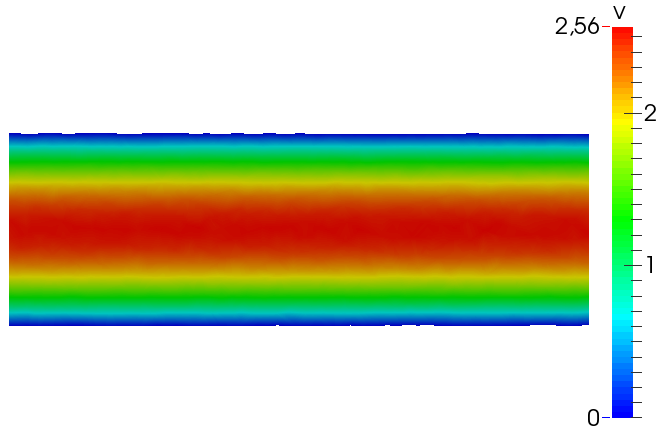
\includegraphics[width=\textwidth]{fig/channel_velocity_step5.png}
\end{minipage}
\hspace{1cm}
\begin{minipage}{0.4\textwidth}
  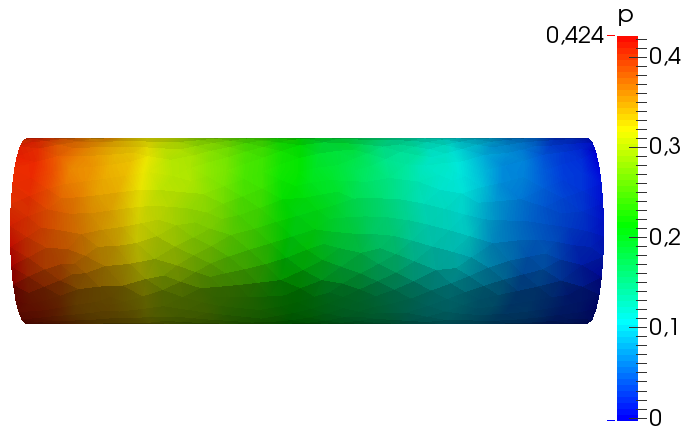
\includegraphics[width=\textwidth]{fig/channel_pressure_step5.png}
  \end{minipage}
\caption{3D channel: laminar constant flow, Poiseuille profile (left), pressure gradient (right).}
 \label{channel}
\end{figure}

\subsection{Example: Cylindrical Channel}\label{sectionChannel}
If we test our simulation with a simple channel geometry and laminar inflow boundary conditions, we expect to obtain a constant flow according to the Hagen-Poiseuille law:
\begin{align}
Q = \frac{\pi R^4 \Delta P}{8 \rho \nu L},
\end{align}
where $Q$ is the volumetric flow rate, $R$ is the radius, $\Delta P$ is the pressure drop and $L$ the length of 
the channel.
The flow is laminar and the fluid does not accelerate through the pipe.

With this simple example it is easy to check the quantities of laminar blood flow, 
its pressure, velocity and shear stress at the wall. Visualizations are shown in figure \ref{channel}.

\subsection{Example: Aortic Blood Flow}\label{sectionAorta}
In this example, we consider a segmented aortic geometry with one Poiseuille-inflow boundary and three outflow boundaries. 
The two upper carrotid outflows are modeled as Poiseuille boundaries, the abdominal outflow is modeled via the $2$-Element Windkessel model with the peripheral resistance and the arterial compliance (for more details see \cite{laskey}):
\begin{align}
\begin{aligned}
 R=&\ 1.185 \cdot 10^8 \frac{kg}{m^4 \cdot s},\\
 C=&\ 1.37 \cdot 10^{-8} \frac{m^4 \cdot s^2}{kg}.
\end{aligned}
\end{align}

\begin{figure}[H]
\centering
\begin{minipage}{0.45\textwidth}
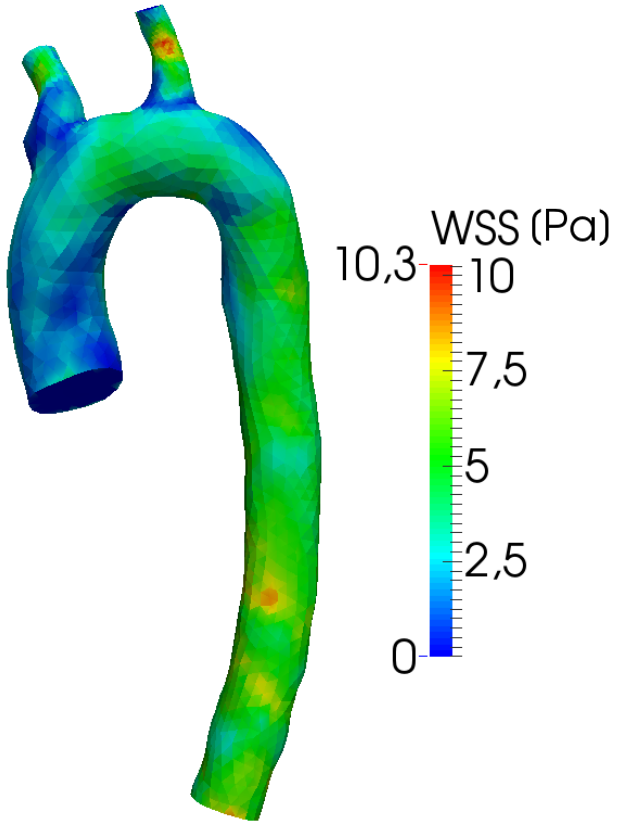
\includegraphics[width=\textwidth]{fig/aorta_wss.png}
\end{minipage}
\hspace{1cm}
\begin{minipage}{0.53\textwidth}
  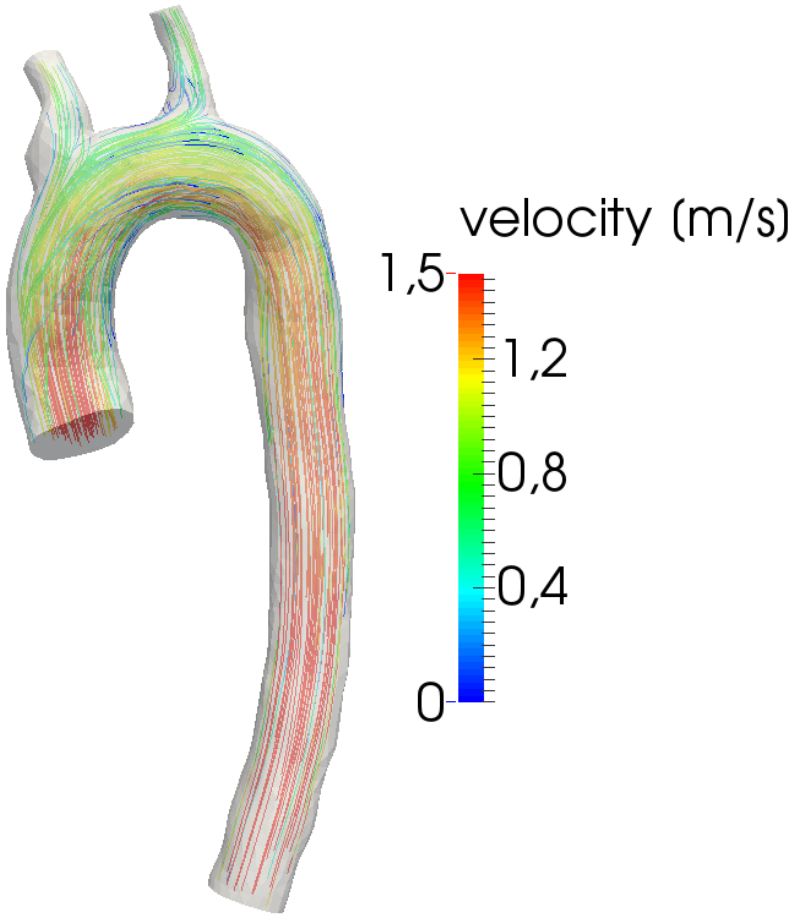
\includegraphics[width=\textwidth]{fig/aorta_streamlines.png}
  \end{minipage}
\caption{Aortic blood flow: Wall shear stress (left) and velocity streamlines (right).}
 \label{aorta}
\end{figure}

Figure \ref{aorta} visualizes the solution at peak systolic blood flow. On the left side you see the shear stresses on the walls of the aorta, calculated via the formula of section \ref{wss}. On the right side the laminar velocity field is shown by means of streamlines.

\newpage
\appendix

\begin{thebibliography}{1}

\bibitem{MPIstandard}
http://www.mcs.anl.gov/research/projects/mpi.

\bibitem{MPI}
William~D. Gropp.
\newblock {\em MPI - Eine Einf\"{u}hrung}.
\newblock Oldenbourg, 2007.

\bibitem{Paraview}
Amy Henderson~Squillacote.
\newblock {\em {The ParaView guide: a parallel visualization application}}.
\newblock Kitware, [Clifton Park, NY], 2007.

\bibitem{tutorial} 
Martin Baumann, A. Helfrich-Schkarbanenko, E. Katelaer, S. Ronnas, Martin Wlotzka. 
\newblock {\em {Boundary Value Problem for Incompressible Navier-Stokes Equation.}}
\newblock Tutorial July, 2014.

\bibitem{cardio} 
Luca Formaggia, Alfio Quarteroni, Alessandro Veneziani. 
\newblock {\em {Cardiovascular Mathematics: Modeling and simulation of the circulatory system.}}
\newblock Springer, 2009.

\bibitem{bcpaper} 
Joao Janela, Alexandra Moura, Adelia Sequeira. 
\newblock {\em {Absorbing boundary conditions for a 3D non-Newtonian fluid structure
interaction model for blood flow in arteries.}}
\newblock Paper, Beng 221-Mathematical Methods in Bioengineering Report, 2012.

\bibitem{windkessel} 
Marianne Catanho, Mridu Sinha, Varsha Vijayan. 
\newblock {\em {Model of Aortic Blood Flow Using the Windkessel Effect.}}
\newblock Paper, International Journal of Engineering Science 48, October 25, 2010.

\bibitem{rannacher} 
Rolf Rannacher. 
\newblock {\em {Finite Element Methods for the Incompressible Navier-Stokes Equations.}}
\newblock Oberwolfach-Seminar, August 11, 1999.

\bibitem{laskey}
Warren K. Laskey, et al.
\newblock {\em {Estimation of total systemic arterial compliance in humans.}}
\newblock Journal of Applied Physiology 69.1, August, 1990.
\end{thebibliography}

%\printindex

\end{document}
